\section{Gipuma}

\textbf{Massively Parallel Multiview Stereopsis by Surface Normal Diffusion}\footnote{\url{https://www.cv-foundation.org/openaccess/content_iccv_2015/papers/Galliani_Massively_Parallel_Multiview_ICCV_2015_paper.pdf}} 这个文章主要在PatchMatch Stereo基础上解决了两个问题(Github\footnote{\url{https://github.com/kysucix/gipuma}}):

\begin{itemize}
	\item 使得PatchMatch Stereo可以并行计算
	\item 扩展PatchMatch Stereo到多视图
\end{itemize}

\subsection{并行计算}

基本思想是把图片上的点分为红黑两组,组内并行计算,组间交替执行,如下图

\begin{figure}[H]
	\begin{center}
		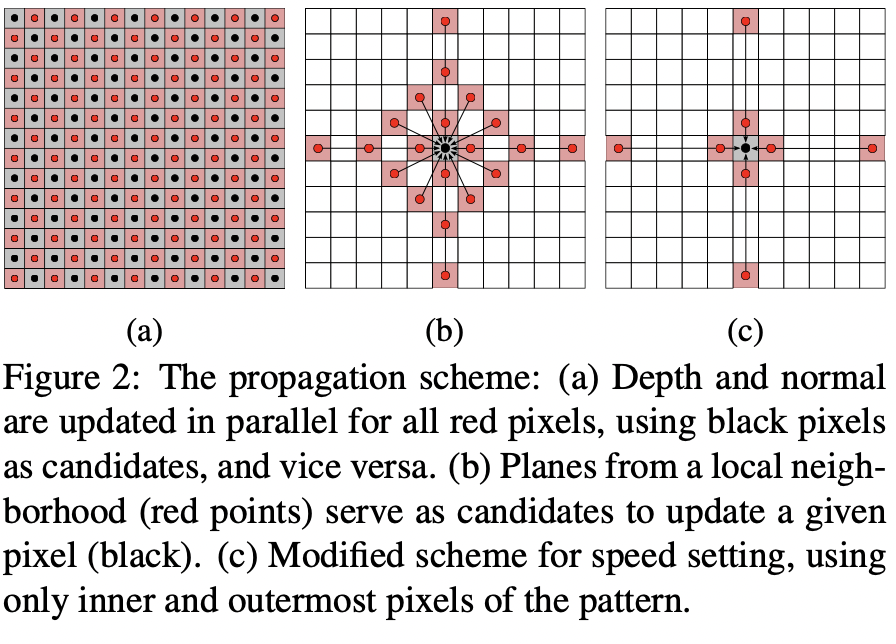
\includegraphics[width=0.8\textwidth]{../images/parallel_compute.png}
	\end{center}
	\caption{Read-Block Group}
\end{figure}

同时还作了一些Sparse Census Transform,使得计算性能很高。

\subsection{多视图支持}

\subsubsection*{修正Z坐标}

在PatchMatch Stereo中作者经常弄混二维坐标、齐次坐标及3D坐标之间的关系,导致深度离散时的坐标$(x_0,y_0,z_0)$并不正确,本文也观察到这一点,所以首先修正Z坐标,

相机内参矩阵,$c,\alpha,u,v$均为内参数,

$$
	\mathbf{K} = \begin{bmatrix}
		c\quad& 0\quad& u\\
		0\quad& c/\alpha\quad& v\\
		0\quad& 0\quad& 1
	\end{bmatrix}
$$

图像点$\mathbf{x}=[x,y]^T$,3D点$\mathbf{X}=[X,Y,Z]^T$,则$\mathbf{x} = \mathbf{K}\mathbf{X}$,

$$
	Z = \frac{-dc}{[x-u,\alpha(y-v),c]\cdot\mathbf{n}}
$$

这个是怎么来的呢?根据$\mathbf{x} = \mathbf{K}\mathbf{X}$,可得,

\begin{align*}
	X &= \frac{(x-v)Z}{c}\\
	Y &= \frac{\alpha yZ}{c}
\end{align*}

代入视差平面方程,$d$为视差
$$
	[X,Y,Z]\cdot \mathbf{n} = -d
$$

则可得出上述表达式。\\

这个表示非常不优雅,实际把$\mathbf{x}$反投影回3D点,尺度为$Z$,反投影的点又在视差平面上,则
$$
	\mathbf{n}^T\cdot Z \mathbf{K}^{-1}\begin{bmatrix*}
		\mathbf{x}\\
		1
	\end{bmatrix*}=-d
$$

可得深度表示,
$$
	Z = -\frac{d}{\mathbf{n}^T\cdot \mathbf{K}^{-1}[\mathbf{x},1]^T}
$$

根本就不需要考虑内参矩阵的具体形式,至此实际建立了视差与深度之间的关系,在此基础上离散深度效果会更好。

\subsubsection*{单应变换}

PatchMatch Stereo需要先对两张图片做视差校准,获得平行水平扫描线才能寻找对应点,本文认为直接通过单应变换查找对应点即可,无需显式构建扫描线,这是一个更深入的洞察。

\subsubsection*{法向量采样}

关于法向量采样,摈弃掉之前粗暴离散化的方法,而是采用半球上的均匀分布,进行采样。\\

通过一个小球面拟合场景曲面的局部更合理,随机取值结果并不是球面上的均匀分布,因此需用专门的采用方法,这里就不再详细介绍。\\

具体操作是,在$(-1,1)$上均匀采样两个点$q_1,q_2$,满足$S = q_1^2 + q_2^2 < 1$,构造法向量,
$$
	\mathbf{n} = \left[1-2S, \quad 2q_1\sqrt{1-S},\quad 2q_2\sqrt{1-S}\right]^T
$$

\subsubsection*{代价聚合}
扩展到多视图,需要选择一张图片做参考,与其他图像之间两两计算cost,N张图片产生N个cost(包括与自身的比较);不是所有目标图像都需要,文中给出一个视角区间,排除那些基线过小或过大的图片。\\

在cost聚合阶段,主要是参考了\textbf{Handling occlusions in dense multi-view stereo},主要是假设一个点能被50\%的图像看到,所以取前只用前50\% cost即够了;但本文实际只用了前3个cost。\\

然后将多个cost作平均得到最终深度图,再通过重投影剔除一些噪音点,包括:
\begin{itemize}
	\item 将N张图片轮番作为参考图计算3D点云
	\item 将3D点投影到$N-1$张图像,得到像素坐标和视差,并检测视差变化是否在某个阈值内
	\item 检测当前点的法向量变化是否在某个阈值内(30°)
\end{itemize}

Gipuma虽然是在PatchMatch Stereo基础上的工作,但无论是计算性能还是建模效果都表现非常不错,后续文献也表面,在DTU数据集上,很少有算法能超过Gipuma的Accuracy指标,包括一些深度学习算法,并且差距还不小。
